\documentclass[serif]{beamer}
% \documentclass[pdf]{beamer}
% \mode<presentation>

%%
%% Generated by Rodrigo Platte, Arizona State University, May 18 2007 %%
%% Edit this file to change how your presentation looks!
%%
%% For more information, please read the manual: beameruserguide.pdf
%%	 

% Select a theme
%%%%%%%%%%%%%%%%%%%%%%%%%%%
  % \usetheme{Montpellier}
  % \usetheme{Ilmenau}
  % \usetheme{Dresden}
  % \usetheme{Frankfurt}
  % \usetheme{Singapore}
  \usetheme{Madrid}
  % \usetheme{Antibes}
  % \usetheme{Berkeley}
  % \usetheme{default}
%%%%%%%%%%%%%%%%%%%%%%%%%%%

% Select a color theme
%%%%%%%%%%%%%%%%%%%%%%%%%%%
  % \usecolortheme{fly}
  \usecolortheme{seagull}
  % \usecolortheme{crane}
  % \usecolortheme{default}
  % \usecolortheme[rgb={.4,0,0}]{structure} % Red colors
  % \usecolortheme[rgb={.2,0,0}]{structure} % Dark Red colors
  % \usecolortheme[rgb={.6,.5,.2}]{structure} % Yellow/Green colors
%%%%%%%%%%%%%%%%%%%%%%%%%%%
  
 % Select a font theme
 %%%%%%%%%%%%%%%%%%%%%%%%%%
  \usefonttheme{structurebold}
  %  \usefonttheme{structuresmallcapsserif}
  % \usefonttheme{structureitalicserif}
  % \usefonttheme{serif}
 %%%%%%%%%%%%%%%%%%%%%%%%%%

 % Select a background color  
 %%%%%%%%%%%%%%%%%%%%%%%%%%%%%%
  \setbeamertemplate{background canvas}[vertical shading][bottom=white,top=gray!30]
  % \setbeamertemplate{background canvas}[vertical shading][bottom=white,top=red!10!black!30]
  %\setbeamertemplate{background canvas}[vertical shading][bottom=white,top=green!20!black!30]
  % \setbeamertemplate{background canvas}[vertical shading][bottom=white,top=white]
%%%%%%%%%%%%%%%%%%%%%%%%%%%%%%%

% Select a color for math text
%%%%%%%%%%%%%%%%%%%%%%%%%%%%%%% 
% \setbeamercolor{math text}{fg=red!80!black}
%%%%%%%%%%%%%%%%%%%%%%%%%%%%%%%


% This command suppresses the navigation symbols at footline
% comment the command below if you  want navigation symbols 
\setbeamertemplate{navigation symbols}{}

% Set the size of the font in frame title
\setbeamerfont{frametitle}{size=\normalsize}


% This command will generate a gray footline with the ASU logo in
% each frame
\useoutertheme{mathASUlogo}
					                                         %

\usepackage[utf8]{inputenc}
\usepackage[T1]{fontenc}

\usepackage{mathpazo}
% \usepackage{pxfonts}
% \usepackage{eulervm}
% \usepackage{bookman}
% \usepackage{times}

\usepackage{xcolor}
\newcommand{\highlight}[1]{%
  \colorbox{red!50}{$\displaystyle#1$}}

\usepackage[spanish]{babel}

\usepackage{physics}

\usepackage{cancel}


\graphicspath{{figuras/}{./}}



\title[Mecánica Newtoniana]{Mecánica general\\[0.5cm] {\Huge Mecánica Newtoniana}}
\author[V. A. Bettachini]{\emph{Víctor A. Bettachini} }
\date{}
% \date{2.o cuatrimestre 2020}
\institute{

\includegraphics[height=1.9cm]{unlam}
\hspace{0.2cm}

\includegraphics[height=1.9cm]{diit}
}


\begin{document}


%%% Title frame %%%%%
\begin{frame}[plain]
	\titlepage
	\transboxout
\end{frame}


\section{Magnitudes vectoriales}

\begin{frame}{Un repaso sobre vectores}

\begin{block}{}
\[
	\vec{r}= r \hat{r}
\]
El vector \(\vec{r}\) tiene
\begin{itemize}
\item un módulo \(r= |\vec{r}|\),
\item y una dirección y sentido denotado por un versor \(\hat{r}\).
\end{itemize}
\end{block}
\pause 

\begin{block}{Operación producto}
\begin{itemize}
	\item por un escalar: \(c \vec{r}= c r_i \hat{i} + c c_j \hat{j}+ c r_k \hat{k}\)
	\item escalar: \(\vec{r} \vec{s} = r s \cos(\theta) = r_i s_i+ r_j s_j + r_k s_k \)
	\begin{itemize}
		\item así el módulo es \(r = |\vec{r}| = \sqrt{\vec{r} \vec{r}}\) 
	\end{itemize}
	\item vectorial: \(\vec{r} \cross \vec{s} = \mdet{
	\hat{i} & \hat{j} & \hat{k} \\
	r_i & r_j & r_k\\
	s_i & s_j & s_k
	}
	\)
\end{itemize}
\end{block}
\end{frame}




\begin{frame}
\begin{block}{Vector posición}
\begin{columns}[c]
      \begin{column}{0.65\textwidth}
        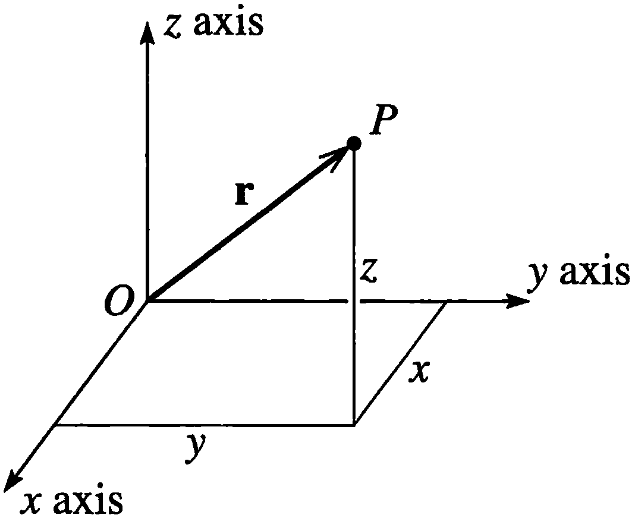
\includegraphics[width=\textwidth]{taylor1_1}
        \end{column}
        \begin{column}{0.35\textwidth}
En coordenadas cartesianas: \(x,y,z\)
\[
\vec{r}= x \hat{x}+ y \hat{y}+ z \hat{z}
\]
\pause
- \(y\) componente de coordenada\\
- \(\hat{y}\) versor de cada eje\\
\bigskip
\pause
A veces se sintetiza
\(\vec{r}= (x,y,z)\)
\end{column}
\end{columns}
\end{block}
\pause
\begin{block}{}
En general: \(\vec{r}= r_1 \hat{e}_1 +  r_2 \hat{e}_2 + r_3 \hat{e}_3\) con \(\hat{e}_i\) de cada sistema de coordenadas.
Por ahora seguimos con cartesianas.
\end{block}
\end{frame}


\begin{frame}{Operando con vectores}
	\begin{block}{Operación suma}
		\[
			\vec{a}= a_i \hat{i} + a_j \hat{j}+ a_k \hat{k}
		\]
		\[
			\vec{b}= b_i \hat{i} + b_j \hat{j}+ b_k \hat{k}
		\]
		\[
			\vec{c} = \vec{a} + \vec{b} = (a_i+b_i) \hat{i} + (a_j+b_j) \hat{j}+ (a_k+c_k) \hat{k}
		\]
	\end{block}

\pause 

\begin{block}{Operación producto}
\begin{itemize}
	\item por un escalar: \(c \vec{r}= c r_i \hat{i} + c c_j \hat{j}+ c r_k \hat{k}\)
	\pause 
	\item escalar: \(\vec{r} \vec{s} = r s \cos(\theta) = r_i s_i+ r_j s_j + r_k s_k \)
	\begin{itemize}
		\item así el módulo es \(r = |\vec{r}| = \sqrt{\vec{r} \vec{r}}\) 
	\end{itemize}
	\pause 
	\item vectorial: \(\vec{r} \cross \vec{s} = \mdet{
	\hat{i} & \hat{j} & \hat{k} \\
	r_i & r_j & r_k\\
	s_i & s_j & s_k
	}
	= (r_j s_k - r_k s_j) \hat{i} + (r_k s_i - r_i s_k) \hat{j} + (r_i s_j - r_j s_i) \hat{k} 
	\)
\end{itemize}
\end{block}
\end{frame}



\begin{frame}
\begin{block}{Velocidad}
\onslide<1->{
\[
\vec{v}= \dot{\vec{r}}= \dv{\vec{r}}{t}= \dv{t}\left( r \hat{r}\right)
\]
}
\onslide<2->{
\[
% \vec{v}= \dot{\vec{r}}= \dv{\vec{r}}{t}=
\vec{v}= \dv{x}{t} \hat{x}+ x \dv{\hat{x}}{t} + 
\dv{y}{t} \hat{y}+ y \dv{\hat{y}}{t} + 
\dv{z}{t} \hat{z}+ z \dv{\hat{z}}{t}
\]
Tendríamos seis términos según la regla de la cadena.\\
}
\onslide<3->{
Pero \(\hat{x}, \hat{y}, \hat{z}\) no varían con \(t\) y por tanto
\[
\vec{v}= \dot{\vec{r}}= 
\dv{x}{t} \hat{x}+
\dv{y}{t} \hat{y}+
\dv{z}{t} \hat{z}
\]
}
\end{block}

\onslide<4>{
\begin{block}{Aceleración}
\[
\vec{a}= \dv{\vec{v}}{t}= \ddot{\vec{r}}=
\dv[2]{x}{t} \hat{x}+
\dv[2]{y}{t} \hat{y}+
\dv[2]{z}{t} \hat{z}
\]
\end{block}
}
\end{frame}


\section{Leyes de Newton}


\begin{frame}
\begin{block}{1.a ley: inercia}
Si la suma de fuerzas \(\sum \vec{F} = 0\) una partícula se mueve con \(\vec{v}\) constante.
\end{block}
\pause
\begin{block}{2.a ley}
\[
\vec{F}= m \vec{a}
\]
\pause
En términos del momento {\tiny (ímpetu)}  \(\vec{p}= m \vec{v}\)
\[
\vec{F} = m \dot{\vec{v}}= \dot{\vec{p}}\qquad (\dot{m}=0 )
\]
\end{block}
\pause
\begin{block}{3.a ley: acción y reacción}
\begin{columns}[c]
	\begin{column}{0.35\textwidth}
		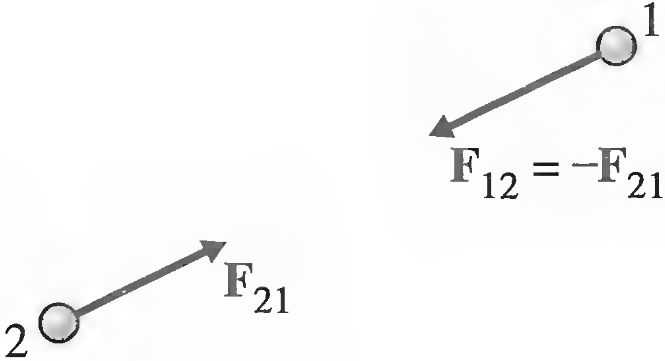
\includegraphics[width=\textwidth]{taylor1_5}
	\end{column}
	\begin{column}{0.65\textwidth}
		Si \textbf{1} ejerce \(\vec{F}_{21}\)  \textbf{2} este ejerce \(\vec{F}_{12}\) a \textbf{1}
		\[
			\vec{F}_{12} = - \vec{F}_{21}
		\]
	\end{column}
\end{columns}
\end{block}

\end{frame}


\begin{frame}
\begin{block}{2.a ley: caso unidimensional}
Para un objeto sobre el eje \(\hat{x}\) sometido a \(\vec{F}= F_o \hat{x}\)
\begin{align*}
\ddot{x}(t)= \frac{F_0}{m}
& \implies \dot{x}(t)= \int \ddot{x}(t) \dd{t} = v_o + \frac{F_0}{m} t \\
& \implies x(t)= \int \dot{x}(t) \dd{t} = x_0 + v_0 t + \frac{F_0}{2 m} t^2
\end{align*}
\pause
\begin{itemize}				
\item<2-> Generando una ecuación diferencial para describir la dinámica, y conociendo \(x_0, v_0\) en \(t_0\), se predicen \(x(t), \dot{x}(t)\) y \(\ddot{x}(t)\).
\item<3-> Esta asignatura apunta a desarrollar la habilidad de modelar con ecuaciones diferenciales la dinámica de sistemas simples.
\item<4-> Posteriores asignaturas (e.g. Estática, Máquinas) aprovechan esta herramienta para el análisis de sistemas mecánicos.
\end{itemize}				
\end{block}
\end{frame}


%\begin{frame}
%\begin{block}{3.a ley: Consevación del momento}
%Si la suma de fuerzas \(\sum \vec{F} = 0\) una partícula se mueve con \(\vec{v}\) constante.
%\end{block}
%\pause
%\begin{block}{2.a ley}
%\(
%\vec{F}= m \vec{a}
%\)
%en terminos del momento \(\vec{p}= m \vec{v}\) (\(\dot{m}=0\)),
%\(
%\vec{F} = \dot{\vec{p}}
%\)
%\end{block}
%\end{frame}


\begin{frame}
\begin{block}{2.a ley en cartesianas: un ejemplo trivial}
\begin{columns}[c]
	\begin{column}{0.35\textwidth}
		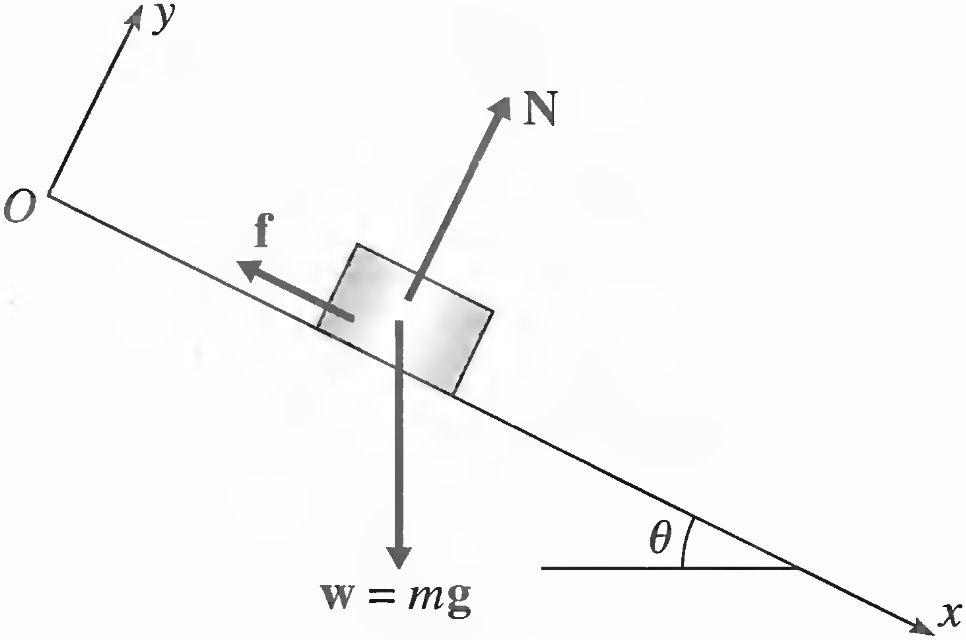
\includegraphics[width=\textwidth]{taylor1_9}
	\end{column}
  \begin{column}{0.65\textwidth}
		\[
		\vec{F}= m \ddot{\vec{x}} \iff
		\begin{cases}
			F_x = m \ddot{x} \\
			F_y = m \ddot{y} \\
			F_z = m \ddot{z}
		\end{cases}
		\]
		\pause
		\begin{align*}
			F_y &= N - \mu m g \cos{\theta} = 0\\
			F_x &= w_x- f = m g \sen{\theta} - \mu m g \cos{\theta} = m \ddot{x}\\
			\ddot{x} &= g \left(\sen{\theta} - \mu \cos{\theta}\right)\\
			x(t) &= \frac{g}{2} \left(\sen{\theta} - \mu \cos{\theta}\right) t^2 \, [\dot{x}(0)=0, x(0)=0]
		\end{align*}
	\end{column}
\end{columns}
\end{block}
\end{frame}


\section{Sistemas de coordenadas}

\begin{frame}
\begin{block}{Coordenadas polares}
\begin{columns}[c]
	\begin{column}{0.35\textwidth}
		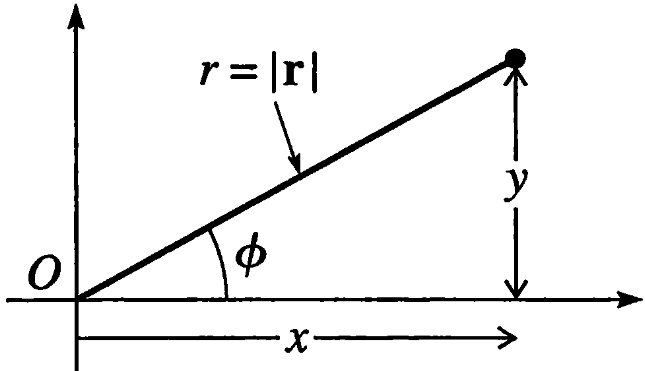
\includegraphics[width=\textwidth]{taylor1_10}
	\end{column}
  \begin{column}{0.65\textwidth}
		\[
		\begin{cases}
			x = r \cos{\phi}  \\
			y = r \sen{\phi}
		\end{cases}
		\iff
		\begin{cases}
			r = \sqrt{x^2+ y ^2} \\
			\phi = \atan{\frac{y}{x}}
		\end{cases}
		\]
	\end{column}
\end{columns}
\end{block}

\pause

\begin{block}{Versor \(\hat{r}\)}
\begin{columns}[c]
	\begin{column}{0.45\textwidth}
		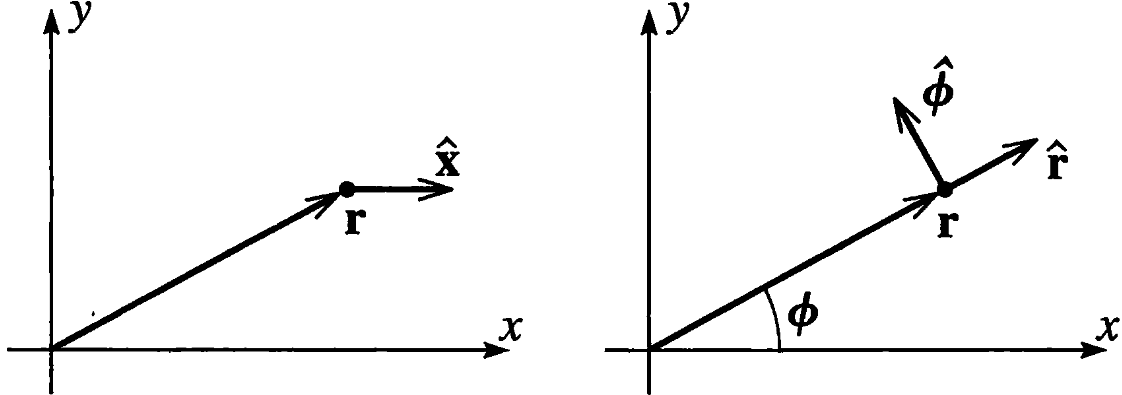
\includegraphics[width=\textwidth]{taylor1_11}
	\end{column}
  \begin{column}{0.55\textwidth}
		\[
		\vec{r}= r \hat{r} \iff \hat{r}= \frac{\vec{r}}{|\vec{r}|}
			\]
		A diferencia de \(\hat{x}\) este versor cambia con el tiempo.
	\end{column}
\end{columns}
\end{block}
\end{frame}


\begin{frame}
\begin{block}{Velocidad en polares}
\begin{columns}[c]
	\begin{column}{0.55\textwidth}
		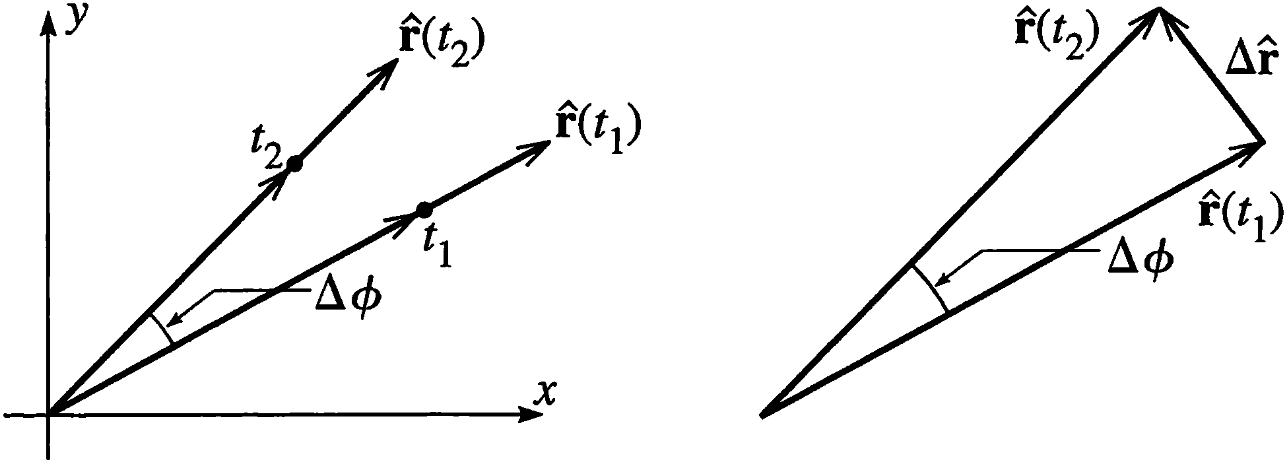
\includegraphics[width=\textwidth]{taylor1_12}
	\end{column}
  \begin{column}{0.45\textwidth}
		\alt<4>{
			\[
				\highlight{
					\dot{\vec{r}}= \dot{r} \hat{r} + r \dot{\phi} \hat{\phi}
				}
			\]
		}
		{
			\[
				\dot{\vec{r}}= \dot{r} \hat{r} + r \dv{\hat{r}}{t}
			\]
		}
		\onslide<2->{
			\[
				\Delta \hat{r} \sim \Delta \phi \hat{\phi} \sim \dot{\phi} \Delta t \hat{\phi}
			\]
		}
		\onslide<3->{
			\[
				\dv{\hat{r}}{t}= \lim_{\Delta t \to 0} \frac{\Delta \hat{r}}{\Delta t} =  \dot{\phi} \hat{\phi}
			\]
		}
	\end{column}
\end{columns}
\end{block}
\end{frame}


\begin{frame}
\begin{block}{Aceleración en polares}
\begin{columns}[c]
	\begin{column}{0.55\textwidth}
		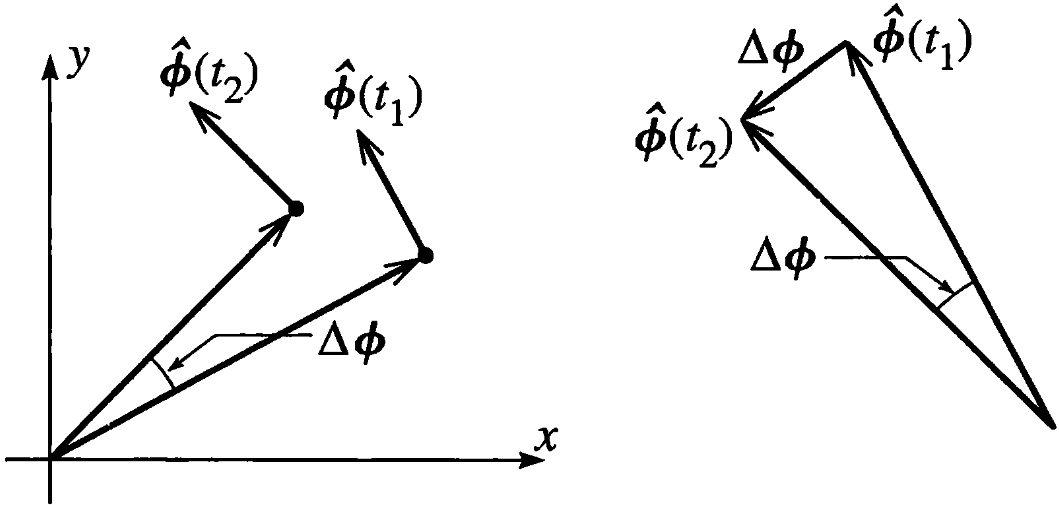
\includegraphics[width=\textwidth]{taylor1_13}
	\end{column}
  \begin{column}{0.45\textwidth}
		\onslide<2->{
		\[
			\dv{\hat{\phi}}{t} = - \dot{\phi} \hat{r}
		\]
		}
		\onslide<3->{
		\begin{align*}
			\vec{a} & = \ddot{\vec{r}}= \dv{\dot\vec{r}}{t}= \dv{t} \left( \dot{r} \hat{r} + r \dot{\phi} \hat{\phi} \right)\\
			& = \left(\ddot{r}- r \dot{\phi}^2 \right) \hat{r}+ \left( r \ddot{\phi} + 2 \dot{r} \dot{\phi} \right) \hat{\phi}
		\end{align*}
		}
	\end{column}
\end{columns}
\end{block}
\end{frame}


\section{Dinámica}


\begin{frame}
\begin{block}{Dinámica de un movimiento circular}
\begin{columns}[c]
	\begin{column}{0.35\textwidth}
		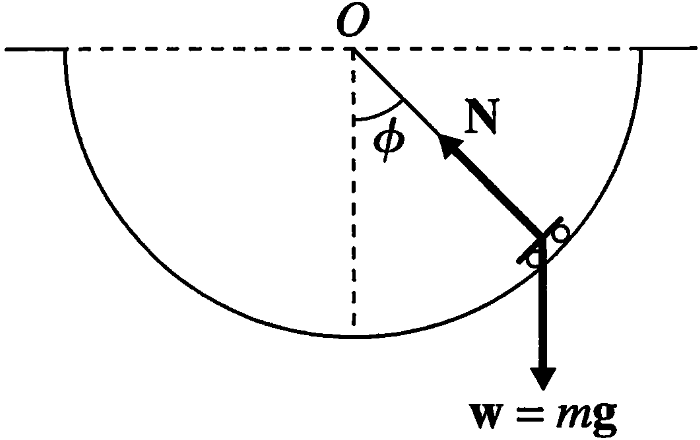
\includegraphics[width=\textwidth]{taylor1_14}
	\end{column}
  \begin{column}{0.65\textwidth}
		\[
			\vec{F}= m \ddot{\vec{r}} \Rightarrow
			\begin{cases}
				F_r = -m R \dot{\phi}^2= m g \cos{\phi} - N \\
				F_\phi = m R \ddot{\phi}= -m g \sen{\phi}
			\end{cases}
		\]
		\pause
		\begin{align*}
			m R \ddot{\phi} & = -m g \sen{\phi} \\
			\ddot{\phi} & = - \frac{g}{R} \sen{\phi} \simeq - \frac{g}{R} \phi\, (\phi \simeq 0)\\
			\phi(t) & = A \sen{\left( \sqrt{\frac{g}{R}} t \right) }+ B \cos(\sqrt{\frac{g}{R}} t) \\
			\omega & =  \sqrt{\frac{g}{R}} \iff T = \frac{2\pi}{\omega}= 2\pi \sqrt{\frac{R}{g}}  
		\end{align*}
	\end{column}
\end{columns}
\end{block}
\end{frame}




\begin{frame}{Movimiento angular} 
\begin{columns}[c]
	\begin{column}{0.35\textwidth}
		\begin{block}{}
			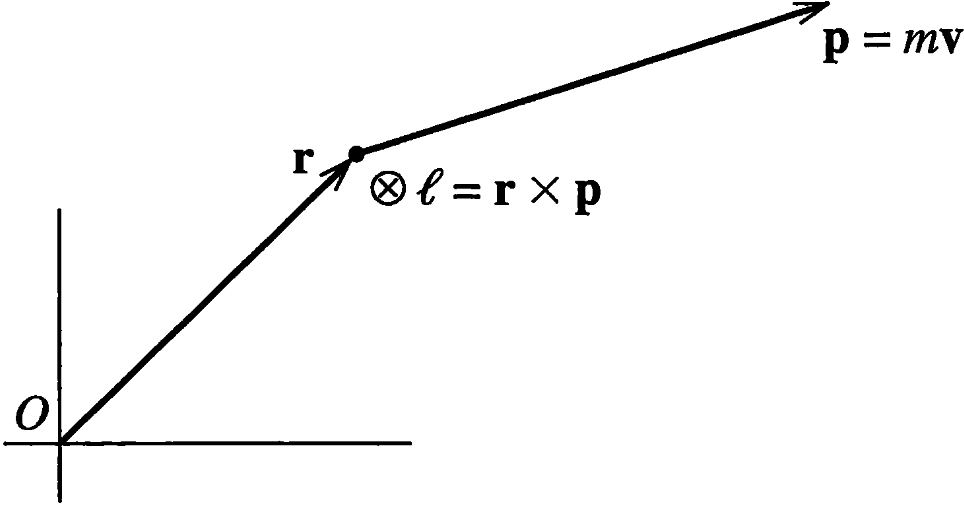
\includegraphics[width=\textwidth]{taylor3_5}
		\end{block}
	\end{column}
  \begin{column}{0.6\textwidth}
		\begin{block}{Momento angular {\tiny (momento cinético)}}
		\[
			\vec{L}=  \vec{r} \cp \vec{p}
		\]
		\end{block}
		\uncover<2>{
		\begin{block}{Torque {\tiny (momento, \(\vec{N}\))}}
		%\alt<2>{
		%\only<2>{
		%	\[
		%		\dot{\vec{L}} = \dot{\vec{r}} \cp \vec{p} + \vec{r} \cp \dot{\vec{p}}
		%	\]
		%}
		%{
			\[
				\dot{\vec{L}} = \cancel{ \dot{\vec{r}} \cp \vec{p}} + \vec{r} \cp \dot{\vec{p}}
			\]
			pues \(\vec{p}= m \dot{\vec{r}} \implies \vec{p} || \dot{\vec{r}} \implies \dot{\vec{r}} \cp \vec{p} = 0 \)
			\pause
			\[
				\vec{\tau} = \dot{\vec{L}}= \vec{r} \cp \vec{F}
			\]
		%}
		\end{block}
		}
	\end{column}
\end{columns}
\end{frame}



\begin{frame}{Movimiento angular}
\begin{columns}[c]
	\begin{column}{0.45\textwidth}
		\begin{block}{Velocidad angular}
		\[
			\dot{\vec{r}} = \dot{r} \hat{r} + r \dot{\phi} \hat{\phi}
		\]
		suele escribirse
		\[ v_r = \dot{r} \quad v_\phi= r \omega \]
		\(v_\phi\): velocidad tangencial
		\end{block}
	\end{column}

	\pause

	\begin{column}{0.45\textwidth}
		\begin{block}{Momento de inercia}
			Para una partícula
			\[
				\vec{L}= \vec{r} \cp m \dot{\vec{r}} = m r^2 \omega= I \omega
			\]
			% \(I\): momento de inercia. 
		\end{block}
	\end{column}
\end{columns}
	
	\pause
	\begin{block}{Momento de inercia de sólidos}
		Para una \(\vec{\omega}= \omega \hat{z}\)
		\[
			I_{zz}= \iiint \rho(x,y,z) \left[ x^2+y^2 \right] \dd{V}
		\]
		Son los elementos diagonales del tensor de inercia \(I_{ij}\).\\
		\pause
		E.g. cilindro | si \(\vec{\omega}= \omega \hat{z}\) (eje) \(I_{zz}= \frac{m}{2}R^2\) | si \(\vec{\omega}= \omega \hat{x}\ \rightarrow I_{xx}= \frac{m}{12} l^2\)
	\end{block}

\end{frame}




\end{document}
